\chapter{Embedding the Simulation Kernel}
\label{cha:embedding}

\section{Architecture}

{\opp} has a modular architecture. The following diagram illustrates  the
high-level architecture of the {\opp} simulations:

\begin{figure}[htbp]
  \begin{center}
    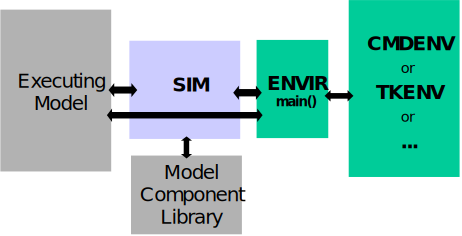
\includegraphics[width=4.757in, height=2.412in]{figures/embed-architecture}
    \caption{Architecture of {\opp} simulation programs}
  \end{center}
\end{figure}

The rectangles in the picture represent the following components:

\begin{itemize}
  \item{\textbf{Sim} is the simulation kernel and class
    library\index{simulation!kernel}. Sim is a library linked to
    your simulation program.}
  \item{\textbf{Envir} is another library containing all the code
    that is common to all the user interfaces. \ffunc{main()} also exists in the Envir library.
    Envir provides services, like ini file handling for specific user interface
    implementations. Envir presents itself towards Sim and the executing model
    via the \ttt{ev} facade object, hiding all other user interface internals.
    Some aspects of the Envir library can be customized\index{customization} using plugin
    interfaces. Embedding {\opp} into applications\index{embedding} can
    be achieved by implementing a new user interface in addition to Cmdenv
    and Tkenv, or by replacing Envir with another implementation of \ttt{ev}
    (see sections \ref{sec:plugin-exts:userinterface} and
    \ref{sec:ch-embedding:embedding}.)}
  \item{\textbf{Cmdenv and Tkenv} are specific user interface
    implementations. The simulation is linked either to the  Cmdenv or Tkenv user interfaces, or to both.}
  \item{The \textbf{Model Component Library} includes simple module definitions and
    their C++ implementations, compound module types, channels, networks,
    message types, and everything belonging to models that
    have been linked to the simulation program. A simulation program can
    run any model that contains all of the required linked components.}
  \item{The \textbf{Executing Model} is the model that is set up
    for simulation. This model contains objects (modules, channels, and so on) that
    are all instances of the components in the model component library.}
\end{itemize}

The arrows in the figure describe how components interact with
each other:

\begin{itemize}
  \item{\textbf{Executing Model $\Leftrightarrow$ Sim}. The simulation kernel
    manages the future events and activates modules in the executing model
    as events occur. The modules of the executing model are stored
    in the main object of Sim, \fvar{simulation} (of class \cclass{cSimulation}).
    In turn, the executing model calls functions in the
    simulation kernel and uses classes in the Sim library.}
  \item{\textbf{Sim $\Leftrightarrow$ Model Component Library}. The simulation kernel
    instantiates simple modules and other components when the simulation model
    is set up at the beginning of the simulation run. In addition, it refers
    to the component library when dynamic module creation is used.
    The mechanisms for registering and looking up components in the model
    component library are implemented as part of Sim.}
  \item{\textbf{Executing Model $\Leftrightarrow$ Envir}. The \ttt{ev} object,
    logically part of Envir, is the facade of the user interface towards the
    executing model. The model uses \ttt{ev} to write debug logs (\ttt{ev<<},
    \ttt{ev.printf()}).}
  \item{\textbf{Sim $\Leftrightarrow$ Envir}. Envir is in full command of what
    happens in the simulation program. Envir contains the \ttt{main()} function
    where execution begins. Envir determines which models should be set up
    for simulation, and instructs Sim to do so. Envir contains the main
    simulation loop (\textit{determine-next-event}, \textit{execute-event}
    sequence) and invokes the simulation kernel for the necessary
    functionality (event scheduling and event execution are implemented in Sim).
    Envir catches and handles errors and exceptions that occur
    in the simulation kernel or in the library classes during execution.
    Envir presents a single facade object (\ttt{ev}) that represents
    the environment (user interface) toward Sim -- no Envir
    internals are visible to Sim or the executing model.
    During simulation model setup, Envir supplies parameter values for
    Sim when Sim asks for them. Sim writes output vectors via Envir,
    so one can redefine the output vector storing mechanism by changing Envir.
    Sim and its classes use Envir to print debug information.}
  \item{\textbf{Envir $\Leftrightarrow$ Tkenv/Cmdenv}. Tkenv and Cmdenv
    are concrete user interface implementations. When a simulation program
    is started, the \ttt{main()} function (which is part of Envir) determines
    the appropriate user interface class, creates an instance and runs it
    by invoking its \ttt{run()} method. Sim's or the model's calls on the
    \ttt{ev} object are delegated to the user interface.}
\end{itemize}


\section{Embedding the {\opp} Simulation Kernel}
\label{sec:ch-embedding:embedding}

This section discusses the issues of embedding the simulation kernel
or a simulation model into a larger application. We assume that you
do not just want to change one or two aspects of the simulator
(such as , event scheduling or result recording) or create a new user interface
such as Cmdenv or Tkenv -- if so, see chapter \ref{cha:plugin-exts}.

For the following section, we assume that you will write the embedding
program from scratch. Meaning, starting from a \ffunc{main()} function.

\subsection{The main() Function}

The minimalistic program described below initializes the simulation library
and runs two simulations. In later sections we will review the details
of the code and discuss how to improve it.

\begin{cpp}
#include <omnetpp.h>

int main(int argc, char *argv[])
{
    // the following line MUST be at the top of main()
    cStaticFlag dummy;

    // initializations
    CodeFragments::executeAll(CodeFragments::STARTUP);
    SimTime::setScaleExp(-12);

    // load NED files
    cSimulation::loadNedSourceFolder("./foodir");
    cSimulation::loadNedSourceFolder("./bardir");
    cSimulation::doneLoadingNedFiles();

    // run two simulations
    simulate("FooNetwork", 1000);
    simulate("BarNetwork", 2000);

    // deallocate registration lists, loaded NED files, etc.
    CodeFragment::executeAll(CodeFragment::SHUTDOWN);
    return 0;
}
\end{cpp}

The first few lines of the code initialize the simulation library. The
purpose of \cclass{cStaticFlag} is to set a global variable to \ttt{true}
for the duration of the \ttt{main()} function, to help the simulation
library handle exceptions correctly in extreme cases.
\ttt{CodeFragment::executeAll(CodeFragment::STARTUP)} performs various startup 
tasks, such as building registration tables out of the \fmac{Define\_Module()},
\fmac{Register\_Class()} and similar entries throughout the code.
\ttt{SimTime::setScaleExp(-12)} sets the simulation time resolution to
picoseconds; other values can be used as well, but it is mandatory to
choose one.

\begin{note}
The simulation time exponent cannot be changed at a later stage, since it is
a global variable, and the values of the existing \ttt{simtime\_t} instances
would change.
\end{note}

The code then loads the NED files from the \ttt{foodir} and
\ttt{bardir} subdirectories of the working directory (as if the NED path
was \ttt{./foodir;./bardir}), and runs two simulations.


\subsection{The simulate() Function}

A minimalistic version of the \ttt{simulate()} function is shown below.
In order to shorten the code, the exception handling code has been ommited (\ttt{try}/\ttt{catch} blocks)
apart from the event loop. However, every line is marked with ``\ttt{E!}'' where various
problems with the simulation model can occur and can be thrown as exceptions.

\begin{cpp}
void simulate(const char *networkName, simtime_t limit)
{
    // look up network type
    cModuleType *networkType = cModuleType::find(networkName);
    if (networkType == NULL) {
        printf("No such network: %s\n", networkName);
        return;
    }

    // create a simulation manager and an environment for the simulation
    cEnvir *env = new CustomSimulationEnv(argc, argv, new EmptyConfig());
    cSimulation *sim = new cSimulation("simulation", env);
    cSimulation::setActiveSimulation(sim);

    // set up network and prepare for running it
    sim->setupNetwork(networkType); //E!
    sim->startRun(); //E!

    // run the simulation
    bool ok = true;
    try {
        while (sim->getSimTime() < limit) {
            cSimpleModule *mod = sim->selectNextModule(); //E!
            if (!mod)
                break;
            sim->doOneEvent(mod);  //E!
        }
        printf("Finished: time limit reached\n");
    }
    catch (cTerminationException& e) {
        printf("Finished: %s\n", e.what());
    }
    catch (std::exception& e) {
        ok = false;
        printf("ERROR: %s\n", e.what());
    }

    if (ok)
        simulation.callFinish();  //E!

    // finish the simulation and clean up the network
    sim->endRun();  //E!
    sim->deleteNetwork();  //E!

    cSimulation::setActiveSimulation(NULL);
    delete sim; // deletes env as well
}
\end{cpp}

The function accepts a network type name (which must be fully qualified
with a package name) and a simulation time limit.

In the first few lines the system looks up the network name among the modules that
have been loaded from the  NED files, and an error message is printed if it is not found.

Then it is required to create and activate a simulation manager object
(\cclass{cSimulation}).
The simulation manager requires another object, called the environment object. This environment object is used by the simulation manager
to read the configuration. In addition, the results produced by the simulation manager are written to this environment object.

The environment object (\ttt{CustomSimulationEnv} in the above code) must
be provided by the programmer; this is described in detail in a later section.

\begin{note}
Before version 4.0, \ttt{simulation} and \ttt{ev} were global variables;
In the current version they are macros that refer to  \ttt{*cSimulation::getActiveSimulation()}
and \ttt{*cSimulation::getActiveSimulation()->getEnvir()}.
\end{note}

The network is then set up in the simulation manager. The
\ttt{sim->}\ffunc{setupNetwork()} method creates the system module and
recursively all modules and their interconnections; module parameters are
also read from the configuration (where required) and assigned. If there is
an error (for example, module type not found), an exception will be thrown. The
exception object is some kind of \cclass{std::exception}, usually a
\cclass{cRuntimeError}.

If the network setup was successful, the \ttt{sim->}\ffunc{startRun()} function is called,
and the \ffunc{initialize()} methods of modules
and channels are then activated. An exception is thrown if
something goes wrong in any of the \ffunc{initialize()} methods.

The following lines run the simulation by calling
\ttt{sim->}\ffunc{selectNextModule()} and \ttt{sim->}\ffunc{doOneEvent()}
in an event loop, until the simulation time limit is reached or an
exception occurs. Exceptions that are subclassed from \cclass{cTerminationException}
signify the normal termination of the simulation process; other exceptions indicate
various errors.

If the simulation has completed successfully (\ttt{ok==true}), the code
goes on to call the \ffunc{finish()} methods of modules and channels. Then,
regardless of whether there was an error, \ttt{sim->}\ffunc{endRun()} is
called, and the network is shut down using
\ttt{sim->}\ffunc{deleteNetwork()}.

Finally, the simulation manager object is deallocated, but the active
simulation manager is not allowed to be deleted; therefore it is deactivated
using \ffunc{setActiveSimulation(NULL)}.


\subsection{Providing an Environment Object}

The environment object needs to be subclassed from the \cclass{cEnvir} class,
but since it has many pure virtual methods, it is easier
to begin by subclassing \cclass{cNullEnvir}. \cclass{cNullEnvir} defines all
pure virtual methods with either an empty body or with a body that throws
an \ttt{"unsupported method called"} exception. You can redefine methods
to be more sophisticated later on, as you progress with the development.

You must redefine the \ffunc{readParameter()} method. This enables
module parameters to obtain their values. For debugging purposes, you can also
redefine \ffunc{sputn()} where module log messages are written to.
\cclass{cNullEnvir} only provides one random number generator, so if your
simulation model uses more than one, you also need to redefine the
\ffunc{getNumRNGs()} and \ffunc{getRNG(k)} methods. To print or store
simulation records, redefine \ffunc{recordScalar()}, \ffunc{recordStatistic()}
and/or the output vector related methods. Other \cclass{cEnvir} methods
are invoked from the simulation kernel to inform the environment about
messages being sent, events scheduled and cancelled, modules created, and so on.

The following example shows a minimalistic environment class that is enough
to get started:

\begin{cpp}
class CustomSimulationEnv : public cNullEnvir
{
  public:
    // constructor
    CustomSimulationEnv(int ac, char **av, cConfiguration *c) :
        cNullEnvir(ac, av, c) {}

    // model parameters: accept defaults
    virtual void readParameter(cPar *par) {
        if (par->containsValue())
            par->acceptDefault();
        else
            throw cRuntimeError("no value for %s", par->getFullPath().c_str());
    }

    // send module log messages to stdout
    virtual void sputn(const char *s, int n) {
        (void) ::fwrite(s,1,n,stdout);
    }
};
\end{cpp}


\subsection{Providing a Configuration Object}

The configuration object needs to subclass from \cclass{cConfiguration}.
\cclass{cConfiguration} also has several methods, but the typed ones
(\ffunc{getAsBool()}, \ffunc{getAsInt()}, etc.) have default implementations
that delegate to the much fewer string-based methods (\ffunc{getConfigValue()}, etc.).

It is fairly straightforward to implement a configuration class that
emulates an empty ini file:

\begin{cpp}
class EmptyConfig : public cConfiguration
{
  protected:
    class NullKeyValue : public KeyValue {
      public:
        virtual const char *getKey() const {return NULL;}
        virtual const char *getValue() const {return NULL;}
        virtual const char *getBaseDirectory() const {return NULL;}
    };
    NullKeyValue nullKeyValue;

  protected:
    virtual const char *substituteVariables(const char *value) {return value;}

  public:
    virtual const char *getConfigValue(const char *key) const
        {return NULL;}
    virtual const KeyValue& getConfigEntry(const char *key) const
        {return nullKeyValue;}
    virtual const char *getPerObjectConfigValue(const char *objectFullPath,
        const char *keySuffix) const {return NULL;}
    virtual const KeyValue& getPerObjectConfigEntry(const char *objectFullPath,
        const char *keySuffix) const {return nullKeyValue;}
};
\end{cpp}


\subsection{Loading NED Files}

NED files can be loaded with any of the following static methods of
\cclass{cSimulation}: \ffunc{loadNedSourceFolder()}, \ffunc{loadNedFile()},
and \ffunc{loadNedText()}. The first method loads an entire subdirectory tree,
the second method loads a single NED file, and the third method takes a literal
string containing NED code and parses it.

\begin{note}
One use of \ffunc{loadNedText()} is to parse NED sources previously converted
to C++ string constants and linked into the executable. This enables
creating executables that are self-contained, and do not require NED files
to be distributed with them.
\end{note}

The above functions can also be mixed, but after the last call,
\ffunc{doneLoadingNedFiles()} must be invoked (it checks for unresolved
NED types).

Loading NED files has a global effect; therefore they cannot be unloaded.


\subsection{How to Eliminate NED Files}

It is possible to get rid of NED files altogether. This would also
remove the dependency on the \ttt{oppnedxml} library and the code in
\ttt{sim/netbuilder}, although at the cost of additional coding.

\begin{note}
When the only purpose is to get rid of NED files as external dependency
of the program, it is simpler to use \ffunc{loadNedText()} on NED files
converted to C++ string constants instead.
\end{note}

The trick is to write \cclass{cModuleType} and \cclass{cChannelType} objects
for your simple module, compound module and channel types, and register them
manually. For example, \cclass{cModuleType} has pure virtual methods called
\ffunc{createModuleObject()}, \ffunc{addParametersAndGatesTo(module)},
\ffunc{setupGateVectors(module)}, \ffunc{buildInside(module)}, which you
need to implement. The body of the \ffunc{buildInside()} method would
be similar to C++ files generated by \fprog{nedtool} of {\opp} 3.x.


\subsection{Assigning Module Parameters}

As already mentioned, modules obtain values for their input parameters
by calling the \ffunc{readParameter()} method of the environment object
(\cclass{cEnvir}).

\begin{note}
\ffunc{readParameter()} is only called for parameters that have not
been set to a fixed (i.e. non-\ttt{default}) value in the NED files.
\end{note}

The \ffunc{readParameter()} method should be written in a manner that enables it to assign
the parameter. When doing so, it can recognize the parameter from its name
(\ttt{par->getName()}), from its full path (\ttt{par->getFullPath()}),
from the owner module's class (\ttt{par->getOwner()->getClassName()})
or NED type name (\ttt{((cComponent *)par->getOwner())->getNedTypeName()}).
Then it can set the parameter using one of the typed setter methods
(\ffunc{setBoolValue()}, \ffunc{setLongValue()}, etc.), or set it
to an expression provided in string form (\ffunc{parse()} method).
It can also accept the default value if it exists (\ffunc{acceptDefault()}).

The following code is a straightforward example that answers parameter
value requests from a pre-filled table.

\begin{cpp}
class CustomSimulationEnv : public cNullEnvir
{
  protected:
    // parameter (fullpath,value) pairs, needs to be pre-filled
    std::map<std::string,std::string> paramValues;
  public:
    ...
    virtual void readParameter(cPar *par) {
        if (paramValues.find(par->getFullPath())!=paramValues.end())
            par->parse(paramValues[par->getFullPath()]);
        else if (par->containsValue())
            par->acceptDefault();
        else
            throw cRuntimeError("no value for %s", par->getFullPath().c_str());
    }
};
\end{cpp}


\subsection{Extracting Statistics from the Model}

There are several ways you can extract statistics from the
simulation.

\subsubsection{C++ Calls into the Model}

Modules in the simulation are C++ objects. If you add the appropriate
public getter methods to the module classes, you can call them from your
main program to obtain statistics. Modules may be looked up with the
\ffunc{getModuleByPath()} method of \cclass{cSimulation}, then cast to the
specific module type via \ffunc{check\_and\_cast<>()} so that the getter
methods can be invoked.

\begin{cpp}
cModule *mod = simulation.getModuleByPath("Network.client[2].app");
WebApp *appMod = check_and_cast<WebApp *>(mod);
int numRequestsSent = appMod->getNumRequestsSent();
double avgReplyTime = appMod->getAvgReplyTime();
...
\end{cpp}

The drawback of this approach is that getters need to be added manually
to all affected module classes, which might not be practical, especially
if modules come from external projects.

\subsubsection{\cclass{cEnvir} Callbacks}

A more general way is to catch \ffunc{recordScalar()} method calls in the
simulation model. The \cclass{cModule}'s \ffunc{recordScalar()} method
delegates to the similar function in \cclass{cEnvir}. You may define the
latter function so that it stores all recorded scalars (for example in an
\ttt{std::map}), where the main program can find them later.
Values from output vectors can be captured in a similar manner.

An example implementation:

\begin{cpp}
class CustomSimulationEnv : public cNullEnvir
{
  private:
    std::map<std::string, double> results;
  public:
    virtual void recordScalar(cComponent *component, const char *name,
                              double value, opp_string_map *attributes=NULL)
    {
       results[component->getFullPath()+"."+name] = value;
    }

    const std::map<std::string, double>& getResults() {return results;}
};

...

const std::map<std::string, double>& results = env->getResults();
int numRequestsSent = results["Network.client[2].app.numRequestsSent"];
double avgReplyTime = results["Network.client[2].app.avgReplyTime"];
\end{cpp}

A drawback of this approach is that compile-time checking of statistics names is lost, but
the advantages are that any simulation model can now be used
without changes, and that capturing additional statistics does not require
code modification in the main program.


\subsection{The Simulation Loop}

To run the simulation, the \ffunc{selectNextModule()} and \ffunc{doOneEvent}
methods of \cclass{cSimulation} must be called in a loop:

\begin{cpp}
while (sim->getSimTime() < limit)
{
    cSimpleModule *mod = sim->selectNextModule();
    sim->doOneEvent(mod);
}
\end{cpp}

Depending on the concrete scheduler class, the
\ffunc{selectNextModule()} may return \ttt{NULL}. The default
\cclass{cSequentialScheduler} never returns \ttt{NULL}.

The execution may terminate in various ways. Runtime errors cause a
\cclass{cRuntimeError} (or other kind of \cclass{std::exception}) to be
thrown. \cclass{cTerminationException} is thrown on normal termination
conditions, such as when the simulation runs out of events to process.

You may customize the loop to exit on other termination conditions as well,
such as on a simulation time limit (see above), on a CPU time limit, or when
results reach a required accuracy. It is relatively straightforward to
build in progress reporting and interactivity (start/stop).

Animation can be hooked up to the appropriate callback methods of
\cclass{cEnvir}: \ffunc{beginSend()}, \ffunc{sendHop()}, \ffunc{endSend()},
and others.


\subsection{Multiple, Coexisting Simulations}

It is possible for several instances of \cclass{cSimulation} to coexist,
and also to set up and simulate a network in each instance. However, this
requires frequent use of \ffunc{cSimulation::set\-Active\-Simulation()}.
Before invoking any \cclass{cSimulation} method or module method,
the corresponding \cclass{cSimulation} instance needs to be designated
as the active simulation manager. This is necessary because several models
and simulation kernel methods refer to the active simulation manager
instance via the \fmac{simulation} macro, and it is similar with the
\fmac{ev} macro.

\begin{note}
Before the 4.0 version, \ttt{simulation} and \ttt{ev} were global variables;
in the current version they are macros that refer to \ttt{*cSimulation::getActiveSimulation()}
and \ttt{*cSimulation::getActiveSimulation()->getEnvir()}.
\end{note}

Every \cclass{cSimulation} instance should have its own associated
environment object (\cclass{cEnvir}). Environment objects may not be
shared among several \cclass{cSimulation} instances. The
\cclass{cSimulation}'s destructor also removes the associated
\cclass{cEnvir} instance.

\cclass{cSimulation} instances may be reused from one simulation to another,
but it is also possible to create a new instance for each simulation run.

\begin{note}
It is not possible to run different simulations concurrently from
different theads, due to the use of global variables which are not easy
to eliminate, such as the active simulation manager pointer and the active
environment object pointer. Static buffers and objects (like string pools)
are also used for efficiency reasons in some places inside the simulation
kernel.
\end{note}


\subsection{Installing a Custom Scheduler}

The default event scheduler is \cclass{cSequentialScheduler}. To replace
it with a different scheduler (e.g. \cclass{cRealTimeScheduler} or your
own scheduler class), add a \ffunc{setScheduler()} call into \ttt{main()}:

\begin{cpp}
cScheduler *scheduler = new CustomScheduler();
simulation.setScheduler(scheduler);
\end{cpp}

It is usually not a good idea to change schedulers in the middle of
a simulation, therefore  \ffunc{setScheduler()} may only be called when
no network is set up.


\subsection{Multi-Threaded Programs}

The {\opp} simulation kernel is not reentrant; therefore it must be protected
against concurrent access.


% --------------------
%
% What you will absolutely need for a simulation to run is the Sim library. You
% probably do not want to keep the appearance of the simulation program, so
% you do not want Cmdenv and Tkenv. You may or may not want to keep Envir.
% You can keep Envir if its philosophy and the infrastructure it provides
% (\ffilename{omnetpp.ini}, certain command-line options etc.) fit into your
% design. Then your application, the embedding program will take the place of
% Cmdenv and Tkenv.
%
% If Envir does not fit your needs (for example, you want the model
% parameters to come from a database not from \ffilename{omnetpp.ini}), then you
% have to replace it. Your Envir replacement (the embedding application,
% practically) must implement the \cclass{cEnvir} member functions from
% \ttt{envir/cenvir.h}, but you have full control over the simulation.
%
% Normally, code that sets up a network or builds the internals of a
% compound module comes from compiled NED source.  You may not like the
% restriction that your simulation program can only simulate networks
% whose setup code is linked in. No problem; your program can contain
% pieces of code similar to what is currently generated by nedtool and then
% it can build any network whose components (primarily the simple modules)
% are linked in. Moreover, it is possible to write an integrated environment
% where you can put together a network using a graphical editor and right
% after that you can run it, without intervening NED compilation and
% linkage.
%
%
%
% \section{Sim: the Simulation Kernel and Class Library}
%
% There is little to say about Sim here, since chapters
% \ref{cha:simple-modules} and \ref{cha:the-simulation-library},
% and part of chapter \ref{cha:messages} are all about
% this topic. Classes covered in those chapters are documented
% in more detail in the API Reference generated by Doxygen.
% What we can do here is elaborating on some internals
% that have not been covered in the general chapters.
%
% The source code for the simulation kernel\index{simulation!kernel}
% and class library reside in the \ttt{src/sim/} subdirectory.
%
%
% \subsection{The Global Simulation Object}
%
% The global \ttt{simulation} object is an instance of \cclass{cSimulation}.
% It stores the model, and encapsulates much of the functionality
% of setting up and running a simulation model.
%
% \ttt{simulation} has two basic roles:
%
% \ b e g i n{itemize}
%   \item{it stores modules of the executing model}
%   \item{it holds the future event set (FES\index{FES}) object}
% \end{itemize}
%
% \subsection{The Coroutine Package}
%
% The coroutine package is in fact made up of two coroutine
% packages\index{coroutine}:
%
% \ b e g i n{itemize}
%   \item A portable coroutine package creates all coroutine stacks
%      inside the main stack. It is based on Kofoed's solution\cite{Kofoed95}.
%      It allocates stack by deep-deep recursions and then plays with
%      \ffunc{setjmp()} and \ffunc{longjmp()} to switch from one to another.
%
%   \item On Windows, the Fiber functions (\ffunc{CreateFiber()},
%      \ffunc{SwitchToFiber()}, etc) are used, which are part of
%      the standard Win32 API.
% \end{itemize}
%
% The coroutines are represented by the \cclass{cCoroutine}
% class. \cclass{cSimpleModule} has \cclass{cCoroutine} as one a
% base class.
%
% \section{The Model Component Library}
%
% All model components (simple module definitions and their C++
% implementations, compound module types, channels, networks,
% message types, etc.) that you compile and link into a simulation
% program are registered in the Model Component Library.
% Any model that has all its necessary components in the
% component library of the simulation program can be run by that
% simulation program.
%
% If your simulation program is linked with Cmdenv or Tkenv,
% you can have the contents of its component library printed,
% using the -h switch.
%
% \ b e g i n {commandline}
% $ ./fddi -h
%
% {\opp} Discrete Event Simulation  (C) 1992-2004 Andras Varga
% ...
% Available networks:
%   FDDI1
%   NRing
%   TUBw
%   TUBs
%
% Available modules:
%   FDDI_MAC
%   FDDI_MAC4Ring
%   ...
%
% Available channels:
%   ...
% End run of {\opp}
% \end{commandline}
%
% Information on components are kept on registration lists.
% There are macros for registering components (that is, for adding
% them to the registration lists):
% \ttt{\fmac{Define\_Module()}}, \ttt{\fmac{Define\_Module\_Like()}},
% \ttt{\fmac{Define\_Network()}}, \ttt{\fmac{Define\_Function()}},
% \fmac{Register\_Class()}, and a few others. For components defined
% in NED files, the macro calls are generated by the NED compiler;
% in other cases you have to write them in your C++ source.
%
% Let us see the module registrations as an example. The
%
% \ b e g i n{verbatim}
% Define_Module(FIFO);
% \end{verbatim}
%
% macro expands to the following code:
%
% \ b e g i n{cpp}
% static cModule *FIFO__create(const char *name, cModule *parentmod)
% {
%     return new FIFO(name, parentmod);
% }
%
% EXECUTE_ON_STARTUP( FIFO__mod,
%     modtypes.getInstance()->add(
%        new cModuleType("FIFO","FIFO",(ModuleCreateFunc)FIFO__create)
%     );
% )
% \end{cpp}
%
% When the simulation program starts up, a new \cclass{cModuleType}
% object will be added to the \ttt{modtypes} object, which holds the list
% of available module types. The \cclass{cModuleType} object will act as a factory:
% when its create() method is called it will produce a new module object
% of class \ttt{FIFO} via the above static function \ttt{FIFO\_\_create}.
%
% The \ttt{cModuleType} object also stores the name of the corresponding
% NED module declaration. This makes it possible to add the gates and parameters
% declared in NED to the module when it is created.
%
% The machinery for managing the registration lists are part
% of the Sim library. Registration lists are implemented
% as global objects.
%
% The registration lists are:
%
% \ b e g i n{longtable}{|p{2cm}|p{4,3cm}|p{7.3cm}|}
% \hline
% %% ROW 1
% \tabheadcol
% \textbf{List variable}
% &
% \textbf{Macro/}\linebreak
% \textbf{Objects on list}
% &
% \textbf{Function} \\\hline
% %% ROW 2
% \ttt{networks}
% &
% \ttt{\fmac{Define\_Network()}} \linebreak
% \linebreak
% \ttt{\cclass{cNetworkType}}
% &
% {\raggedright List of available networks\index{network!list of}.
% Every \cclass{cNetworkType} object is a factory for a specific
% network type. That is, a \cclass{cNetworkType} object has methods
% for setting up a specific network.
% \fmac{Define\_Network()} macros occur in the code generated by the NED
% compiler.}\\\hline
% % ROW 3
% \ttt{modtypes}
% &
% \ttt{\fmac{Define\_Module()},} \linebreak
% \ttt{\fmac{Define\_Module\_Like()},}  \linebreak
% \linebreak
% \ttt{\cclass{cModuleType}}
% &
% {\raggedright List of available module types.
% Every \cclass{cModuleType} object is a factory for a specific module
% type. Usually, \fmac{Define\_Module()} macros for compound modules occur in
% the code generated by the NED compiler; for simple modules,
% the \fmac{Define\_Module()} lines are added by the user.}\\\hline
% %% ROW 4
% \ttt{channeltypes}
% &
% \fmac{Define\_Channel()} \linebreak
% \linebreak
% \cclass{cChannelType}
% &
% {\raggedright List of channel types.
% Every \cclass{cChannelType} object acts as a factory for a channel type,
% a class derived from \cclass{cChannel}.} \\\hline
% %% ROW 5
% \ttt{classes}
% &
% \fmac{Register\_Class()} \linebreak
% \linebreak
% \ttt{cClassRegister}
% &
% {\raggedright List of available classes of which one can create
% an instance.
% Every \cclass{cClassRegister} object is a factory for objects
% of a specific class. The list is used by the \ffunc{createOne()} function:
% it can create an object of any class, given the class name as a string.
% (E.g. the statement \ttt{ptr = createOne("cArray")} creates a \ttt{cArray} object.)
% To enable a class to work with \ttt{createOne()}, one has to register it using the
% \ttt{Register\_Class(classname)} macro}\\\hline
% %% ROW 6
% \ttt{functions}
% &
% \ttt{\fmac{Define\_Function()}} \linebreak
% \linebreak
% \ttt{\cclass{cFunctionType}}
% &
% {\raggedright List of functions taking \ttt{double}s and returning a \ttt{double}
% (see type \ttt{MathFuncNoArg}...\ttt{MathFunc3Args}).
% A \cclass{cFunctionType} object holds a pointer to the function and knows
% how many arguments it takes.}\\\hline
% \end{longtable}
%
%
% \section{Envir, Tkenv and Cmdenv}
%
% The source code for the user interface of {\opp} resides in the
% \texttt{src/envir/} directory (common part) and in the \texttt{src/cmdenv/},
% \texttt{src/tkenv/} directories.
%
% The classes in the user interface are \textit{not} derived from \cclass{cOwnedObject},
% they are completely separated from the simulation kernel.
%
%
% \subsection{The main() Function}
%
% The \ffunc{main()} function of {\opp} simply sets up the user
% interface and runs it. Actual simulation is done in
% \ffunc{cEnvir::run()} (see later).
%
%
% \subsection{The cEnvir Interface}
%
% The \cclass{cEnvir} class has only one instance, a global object
% called \fvar{ev}:
%
% \ b e g i n{cpp}
% cEnvir ev;
% \end{cpp}
%
% \cclass{cEnvir} basically a facade, its member functions
% contain little code. \cclass{cEnvir} maintains a pointer to a
% dynamically allocated simulation application object (derived from
% \cclass{TOmnetApp}, see later) which does all actual work.
%
%
% \cclass{cEnvir} member functions perform the following groups of tasks:
% \ b e g i n{itemize}
%   \item I/O for module activities; the actual implementation is different
%     for each user interface (e.g. stdin/stdout for Cmdenv, windowing
%     in Tkenv)
%   \item cEnvir provides methods for the simulation kernel to
%     access configuration information (for example, module parameter settings)
%   \item cEnvir also provides methods that are called by simulation kernel to
%     notify the user interface of certain events (an object was deleted;
%     a module was created or deleted; a message was sent or delivered, etc.)
% \end{itemize}

%%% Local Variables:
%%% mode: latex
%%% TeX-master: "usman"
%%% End:

